\documentclass{article}
\usepackage{graphicx} % Required for inserting images
\usepackage{authblk} 
\usepackage{amsmath} 

\title{Resumen del Capítulo 2 de “Introduction To The Theory of Neural Computation” de Hertz, Krogh y Palmer (1991).}
\author{Rodrigo García Núñez}
\affil{Universidad Autónoma Metropolitana }
\date{Febrero 2025}


\begin{document}

\maketitle

\section{Problema de la memoria Asociativa}

Este capítulo comienza mencionando que la memoria asociativa es la “mosca de la fruta” o
el “átomo de Bohr” en este campo. Se refiere a la forma más simple en la que la
computación colectiva puede trabajar. El problema dice así:
\\
Almacena un conjunto de p patrones $\epsilon^\mu_i$ de tal forma que cuando se le presente un nuevo patrón a la red $\lambda_i$, la red debe responder con cualquiera de los patrones previamente almacenados que sea más cercano a $\lambda_i$.
\\\\
Los patrones son etiquetados por $\mu = 1, 2, ..., p$, mientras que las unidades de la red (neuronas) se identifican con $i= 1, 2, ..., N$. Tanto los patrones almacenados en la red $\epsilon^\mu_i$ como los patrones de prueba $\lambda_i$ pueden ser 0 o 1 en cada unidad $i$. Sin embargo, se nos dice que a continuación se adoptará una convención más cómoda.
\\\\
Claro que aunque esto podría resolverse con un programa que calculase la distancia de Hamming entre un patrón almacenado $\epsilon^\mu_i$ y uno de prueba $\lambda_i$, nos interesa más ver cómo hacer que una red de McCulloch-Pitts adopte el patrón almacenado más cercano al patrón de prueba. Dicho esto, lo que queremos saber es, arrancando de una configuración $n_i = \lambda_i$, qué conjunto de pesos $w_{ij}$ hará que la red adopte el estado en el que $n_i = \epsilon^{\mu_0}_i$. De ese modo, la red será direccionable por contenido y no será afectada en gran medida por pequeños errores del patrón de entrada.
\\\\
Un ejemplo que recupero de capítulo que representa el poder de una red direccionable por contenido es que si tuviéramos una red en la que almacenamos información codificada acerca de varios científicos famosos y le pasáramos de patrón de entrada "evolución" o "$E = mc³$" la red sería capaz de responder Darwin o Einstein, respectivamente, a pesar del error presente en la famosa ecuación.
\\\\
El \textbf{espacio de configuraciones} es representado en la figura 1. Dentro de ese espacio se encuentran los patrones almacenados $\epsilon^\mu_i$ y se les conoce como \textbf{atractores}, los cuales, como indica su nombre, atraen el estado de la red desde un patrón inicial. De este modo, el espacio de configuraciones está dividido por \textbf{zonas de atracción} dados por los diferentes atractores.

\begin{figure}[h]
\centering
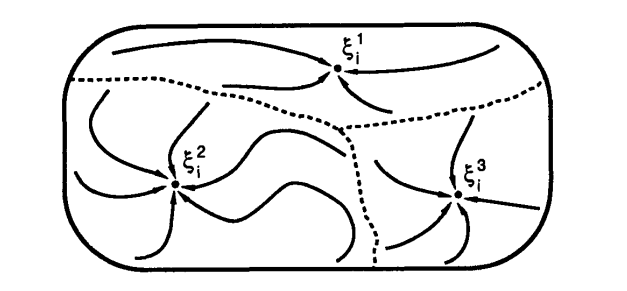
\includegraphics[width=0.5\textwidth]{images/espacioConf.png}
\caption{Espacio de soluciones}
\label{fig:Espacio de soluciones}
\end{figure}
\\


\section{El Modelo}

Como se mencionó anteriormente, desde ahora se usará una convención más cómoda matemáticamente.Ahora, los valores de activación de las neuronas son +1 (disparando) y -1 (no disparando), en lugar de 0 y 1. Ahora, las unidades se denotan con $S_i$ en lugar de $n_i$. La conversión de $n_i = 0 $ o 1 es dada por $S_i = 2n_i - 1$. Con estos cambios, el modelo general de la neurona descrita en el capítulo anterior se escribe así:

\begin{equation}
    S_i := sgn(\sum w_{i,j}S_j - \theta_i)
    \label{eq:Modelo}
\end{equation}
\\\\
Tal que la función umbral sgn(x) será:

\begin{equation}
    sgn(x) =
    \begin{cases}
        1, & \text{si } x \geq 0 \\
        -1, & \text{si } x < 0
    \end{cases}
    \label{eq:umbral sgn}
\end{equation}
\\
Y el umbral $\theta_i$ está asociado con $\mu_i$, descrita en el capítulo anterior, de modo que $\theta_i = 2\mu_i - \sum_j w{ij}$. Sin embargo, por fines prácticos, por el resto del capítulo tendremos que $\theta_i = 0$, tal que nos quedamos con la siguiente representación:

\begin{equation}
    S_i := sgn(\sum w_{i,j}S_j)
    \label{eq:Modelo}
\end{equation}
\\

Hay dos maneras en que podemos trabajar la actualización de las unidades: sincrónica, actualizar todas las unidades simultáneamente, o asincrónica, actualizar una unidad por cada instante. Por un lado, la actualización sincrónica requiere de un sistema extra que marque la pauta para actualizar, lo que vuelve el modelo sensible a errores de sincronización. Por otro lado, la actualización asincrónica es más natural respecto a las neuronas reales y se puede proceder de dos formas:
\begin{itemize}
    \item En cada instante, se selecciona aleatoriamente una unidad i para actualizarla, y aplicar la ecuación 1.
    \item Dejar que cada unidad se actualice independientemente con cierta probabilidad por cada instante.
\end{itemize}
\\

También es necesario especificar después de cuántas actualizaciones le pediremos a la red que devuelva el patrón almacenado más cercano al patrón inicial. En el caso de la actualización sincrónica se puede optar por que el estado inicial de la red alcance el estado almacenado más cercano inmediatamente.  

En este capítulo estudiaremos un problema genérico de un conjunto aleatorio de patrones $\epsilon_i$ de bits que pueden ser valores de +1 o -1. El procedimiento para verificar que los pesos $w_{ij}$ sean aceptables para almacenar patrones es ver si los patrones a almacenar son estables, y después corroborar si, dada alguna desviación en el patrón inicial, es corregida a medida que las unidades se actualizan. 

\section{Un solo patrón a almacenar}

Primero, consideramos el caso básico en el que queremos almacenar en la red un solo patrón $\epsilon_i$. La condición para que ese patrón sea estable es:

\begin{equation}
    sgn(\sum w_{ij}\epsilon_j) = \epsilon_i
    \label{eq:patrón estable}
\end{equation}
\\

pues entonces la ecuación 3 no produce ningún cambio. Esto es verdadero si tenemos que
\begin{equation}
    w_{ij} \propto \epsilon_i \epsilon_j
    \label{eq:prpporcionalidad}
\end{equation}
\\

Por conveniencia, hacemos que la constante de proporcionalidad sea $1/N$, en donde $N$ es el número de unidades que conforman la red. Esto se hace para normalizar los pesos de la red y que no tomen valores disparatados.

\begin{equation}
    w_{ij} = (1/N) \epsilon_i \epsilon_j
    \label{eq:normalización de pesos}
\end{equation}
\\
Notese que si un poco menos de la mitad de los bits  del patrón inicial $S_i$ estuvieran equivocados, estos se verían opacados por la mayoría de bits que sí están bien, por lo que el patrón de la red recaería en el patrón $\epsilon_i$ almacenado, actuando como atractor .
Dicho esto, ¿y si la mayoría de bits del patrón inicial estuvieran mal? En este caso, hay que mencionar que en este caso básico, se hallan dos atractores, $\epsilon_i$ y $-\epsilon_i$, por lo que en el escenario en el que la mayoría de los bits del estado inicial estén mal, la configuración de la red será atraída por el \textbf{estado inverso} $-\epsilon_i$
\\\\
\begin{figure}[h]
\centering
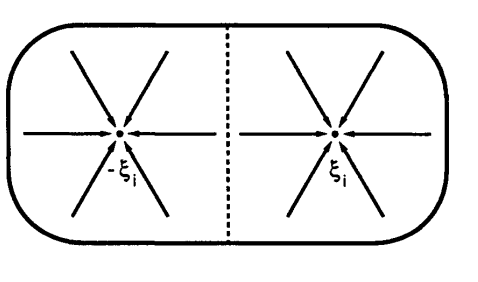
\includegraphics[width=0.5\textwidth]{images/espacio1solopatron.png}
\caption{Espacio de configuraciones con un solo patrón almacenado}
\label{fig:Espacio de soluciones}
\end{figure}
\\\\\

\section{Más de un patrón a almacenar}

Para el caso de tener más de un patrón que quisiéramos almacenar, optamos por hacer a los conjuntos de pesos $w_{ij}$ una superposición de pesos como en la ecuación 6, una para cada patrón, tal que

\begin{equation}
    w_{ij} = (1/N) \sum^p_{\mu=1} \epsilon^\mu_i \epsilon^\mu_j
    \label{eq:regla ded hebb}
\end{equation}
\\
Nótese que en esta ecuación p es el número total de patrones almacenados en la red, etiquetados por $\mu$.
\\\\
A esto se le conoce como "regla de Hebb" dada la similitud entre la ecuación 7 con una hipótesis hecha por Hebb (1949) respecto a cómo cambia la fuerza sináptica (pesos) entre neuronas conforme a la experiencia.
\\\\
Un modelo con memoria asociativa usando la regla de Hebb (ecuación 7) para cada set de pesos $ij$, con unidades binarias y actualización asincrónica, es usualmente llamado \textbf{modelo de Hopfield}. A pesar de que la mayoría de los componentes del modelo ya eran conocidos desde antes, el trabajo de Hopfield (1982) fue lo que los integró, introduciendo una función de energía y la idea de recuerdos o memorias almacenadas como atractores dinámicos.
\\\\

Como en el caso de un solo patrón a almacenar, debemos examinar la estabilidad de un patrón particular $\epsilon_i^v$. La condición de estabilidad se generaliza para todo $i$ a
\begin{equation}
    sgn(h_i^v) = \epsilon_i^v
    \label{eq:condición de estabilidad}
\end{equation}
\\
en donde la entrada $h_i^v$ a la unidad $i$ en el patrón $v$ es
\begin{equation}
    h_i^v \equiv \sum_jw_{ij}\epsilon_j^v = (1/N)\sum_j\sum_\mu\epsilon_i^\mu\epsilon_j^\mu\epsilon_j^v
    \label{eq:condición de estabilidad}
\end{equation}
\\
Ahora se separa la sumatoria de $\mu$ del término en el que $\mu=v$
\begin{equation}
    h_i^v = \epsilon_i^v + (1/N)\sum_j\sum_{\mu\neq v}\epsilon_i^\mu\epsilon_j^\mu\epsilon_j^v
    \label{eq:condición de estabilidad}
\end{equation}
\\
Si el segundo término es cero o lo suficientemente pequeño (menor que 1), entonces, y de acuerdo con la ecuación de estabilidad, el patrón $\epsilon_i^v$ es estable. A este término se le llama \textbf{el término de interferencia} y tiende a ser menor que 1 cuando el número de patrones almacenados es lo suficientemente pequeño.
\\\\
\section{Capacidad de almcenamiento}

Tomando en cuenta la siguiente expresión
\begin{equation}
    C_i^v \equiv  -\epsilon_i^v (1/N)\sum_j\sum_{\mu\neq v}\epsilon_i^mu\epsilon_j^\mu\epsilon_j^v
    \label{eq:condición de estabilidad}
\end{equation}
\\
Esto solo son $-\epsilon_i^v$ veces el término de interferencia en la ecuación 10. Si $C_i^v$ es negativo, entonces el término de interferencia tiene el mismo signo que el patrón deseado $\epsilon_i^v$, por lo que no afecta. Por otro lado, si $C_i^v$ sí es positivo, y mayor que 1, entonces sí cambiará el signo de $h_i^v$ y vuelve al patrón de la unidad i inestable. Si se inicia la red en estado de memoria deseado $\epsilon_i^v$, no se quedará ahí.
\\\\
Ahora, es momento de considerar patrones aleatorios, con igual probabilidad de que $\epsilon_i^v$ sea +1 o -1. Con esto, podemos estimar la probabilidad de que un patrón arbitrario sea inestable. A esta probabilidad la llamamos $P_{error}$ y la representamos de la siguiente forma:
\begin{equation}
    P_{error} =Prob (C_i^v > 1)
    \label{eq:P_{error}}
\end{equation}
\\
Nótese que $P_{error}$ aumenta cuando incrementamos la cantidad de p patrones que queremos almacenar en la red. Para encontrar la máxima cantidad de patrones que podemos almacenar en una red, debemos adoptar un criterio de aceptación de rendimiento, por ejemplo $P_{error} < 0.01$.
\\\\
Cómo se puede apreciar, $P_{error}$ depende de la cantidad de unidades $N$ y $p$, el número de patrones que queremos almacenar. Ahora $C_i^v$ es $1/N$ veces la suma de $Np$ números aleatorios, en donde es igual de posible que sean +1 o -1, como una distribución binomial con promedio 0 y una varianza $\sigma² = p/N$. Sin embargo, asumimos que p y N son grandes, esto podemos aproximarlo como una distribución Gaussiana, con promedio y varianza iguales, como se muestra en la figura 3.

\begin{figure}[h]
\centering
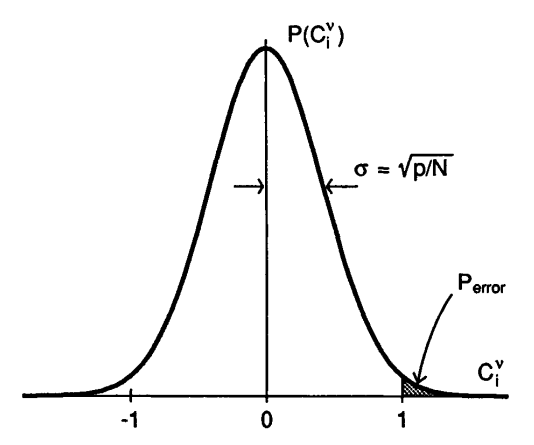
\includegraphics[width=0.5\textwidth]{images/distribusión.png}
\caption{Distribución de los valores del término de interferencia $C_i^v$. Para $p$ patrones aleatorios y $N$ unidades, se obtiene una distribución Gaussiana con varianza $\sigma² = p/N$. Lo sombreado es la probabilidad de error por bit.}
\label{fig:Espacio de soluciones}
\end{figure}


\section{Bibliografía}

\begin{thebibliography}{9}

\bibitem{John H., Anders K. y Richard G. P. (1992)} John H., Anders K. y Richard G. P. (1992). Introduction to the theory of Neural
Computation (pp. 11 - 20). CRC Press.


\end{thebibliography}
\end{document}
